\documentclass{book}

\usepackage{amssymb}
\usepackage{amsmath}
\usepackage{amsthm}
\usepackage{arydshln}
\usepackage{calc}
\usepackage{cancel}
\usepackage{caption}
\usepackage{cite}
\usepackage{color}
\usepackage{enumitem}
\usepackage{esint}
\usepackage{etoolbox}
\usepackage{float}
\usepackage{framed}
\usepackage{fullpage}
\usepackage{gensymb}
\usepackage[margin=1in]{geometry}
\usepackage{graphicx}
\usepackage{listings}
\usepackage{multirow}
\usepackage{subfiles}
\usepackage{rsfso}
\usepackage{tikz}
\usepackage{tikz-3dplot}
\usepackage{ushort}
\usepackage{wrapfig}
\usepackage{xcolor}
\usepackage{soul}
\usepackage{epstopdf}
\usepackage{pdfpages}

% pdf versions
\pdfoptionpdfminorversion=7

% handle page stretching
\raggedbottom

% Graphics file location
\graphicspath{{Graphics/}{../Graphics/}}

% Use for drawings
\usetikzlibrary{angles,arrows,calc,decorations,intersections,patterns,positioning,quotes,shapes}
\usetikzlibrary{shapes.geometric}
\usetikzlibrary{decorations.pathreplacing}
\newcommand{\midarrow}{\tikz \draw[-latex] (0,0) -- +(.1,0);}

% Tikz commands for drawing block diagrams, etc...
\tikzset{%
	block/.style    = {draw, rectangle, minimum height = 2em, minimum width = 2em},
	sum/.style      = {draw, circle}, % Adder
	input/.style    = {fill=white, rectangle}, % Input
	output/.style   = {fill=white, rectangle}, % Output
	waypoint/.style   = {coordinate}, % Output
}

\tikzset{%
	startstop/.style= {draw, rectangle, rounded corners, minimum width=2cm, minimum height=1cm,text centered},
	inout/.style    = {draw, trapezium, trapezium left angle=70, trapezium right angle=110, minimum width=2cm, minimum height=1cm, text centered},
	process/.style  = {draw, rectangle, minimum width=2cm, minimum height=1cm, text centered},
	decision/.style = {draw, diamond, minimum width=1.5cm, minimum height=1cm, text centered, diamond, aspect=2},
	arrow/.style    = {thick,-latex,>=stealth},		
}

\tikzset{
	saveuse path/.code 2 args={
		\pgfkeysalso{#1/.style={insert path={#2}}}%
		\global\expandafter\let\csname pgfk@\pgfkeyscurrentpath/.@cmd\expandafter\endcsname
		% not optimal as it is now global through out the document
		\csname pgfk@\pgfkeyscurrentpath/.@cmd\endcsname
		\pgfkeysalso{#1}},
	/pgf/math set seed/.code=\pgfmathsetseed{#1}}

% Define Laplace, Fourier transform symbols
\newcommand{\LT}{\mathcal{L}}
\newcommand{\FT}{\mathcal{F}}

% Define adjugate function
\newcommand{\adj}{\text{adj}}

% Define rank function
\newcommand{\rank}{\text{rank}}

% commands to speed up writing j\omega and s-plane
\newcommand{\jw}{j\omega}
\newcommand{\spl}{s\textrm{-plane}}
\newcommand{\wt}{\omega t}
\newcommand{\Lm}{\textrm{Lm }}
% Clean up overline/underline for math mode
\def\obar#1{\bar{#1}}
\def\ubar#1{\ushort{#1}}

\newcommand{\exmp}{\subsubsection*{Example}}
\newcommand{\nib}{\noindent$ \bullet\ $}


\begin{document}
\chapter*{Lecture 1}
\section*{Introduction}
The title of this course is \textsc{Automatic Control of Engineering Systems}. The key work here is ``control''. In general, to control something means to get the thing to behave in a certain fashion. From the engineering point of view, ``control'' is the process of causing one or more system variable(s) to conform to some desired value(s) called reference value(s).

Here, a system is a collection of things (by man or nature) that form an integral whole. For example, an automobile, building, airplane, dog, human being, plant, etc... The ``variable'' of interest would depend on the system.

\begin{itemize}
	\item For a building:
	\begin{itemize}
		\item temperature
		\item humidity
		\item etc...
	\end{itemize}
	\item For an airplane:
	\begin{itemize}
		\item temperature inside the cabin
		\item speed of the plane
		\item heading
		\item etc...
	\end{itemize}
	\item For an automobile:
	\begin{itemize}
		\item speed control
		\item yaw control
		\item etc...
	\end{itemize}
\end{itemize}

Control systems can be classified as follows
\begin{center}
	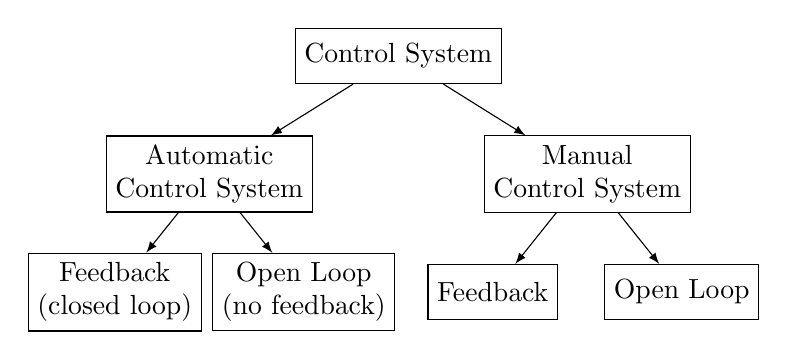
\begin{tikzpicture}[xscale=1.2]
	\node[block] (top) at (0,0) {Control System};
	\node[block,align=center] (midleft) at (-2,-1.5) {Automatic\\Control System};
	\node[block,align=center] (midright) at (2,-1.5) {Manual\\Control System};
	\node[block,align=center] (b1) at (-3,-3) {Feedback\\(closed loop)};
	\node[block,align=center] (b2) at (-1,-3) {Open Loop\\(no feedback)};
	\node[block,align=center] (b3) at (1,-3) {Feedback};
	\node[block,align=center] (b4) at (3,-3) {Open Loop};
	\draw[-latex] (top) -- (midleft);
	\draw[-latex] (top) -- (midright);
	\draw[-latex] (midright) -- (b3);
	\draw[-latex] (midright) -- (b4);
	\draw[-latex] (midleft) -- (b1);
	\draw[-latex] (midleft) -- (b2);
	\end{tikzpicture}
\end{center}

Definitions:
\begin{itemize}
	\item \textbf{Automatic Control System:} completes desired tasks with minimal human intervention
	\item \textbf{Manual Control System:} Needs frequent intervention by humans
\end{itemize}

\textbf{Examples:}
Automatic Control Systems:
\begin{itemize}
	\item Washing machine
	\item Automatic lawn sprinkler
	\item Central heating/air conditioning
	\item Elevators
	\item etc...
\end{itemize}
Manual Control Systems:
\begin{itemize}
	\item Driving a car
	\item Manual lawn sprinkler
	\item Lighting in a house
	\item Space heaters
	\item etc...
\end{itemize}

More definitions:
\begin{itemize}
	\item \textbf{Feedback Control System:} Contains a measurement device (called a sensor) that monitors the variable(s) of interest. The value(s) of these variables are compared to desired values and the difference (if any) is used to ``move'' the control system in one direction or the other.
	\item \textbf{Open-Loop System:} Not equipped with any sensor, so, control action is not based on actual value of output.
\end{itemize}
\textbf{Examples:}
Feedback Control Systems:
\begin{itemize}
	\item Car/Airplane speed control
	\item Central heating/air conditioning
	\item etc...
\end{itemize}
Open-Loop Control Systems:
\begin{itemize}
	\item Automatic lawn sprinkler
	\item Washing machine
	\item Clothes dryer
	\item etc...
\end{itemize}

In summary, we have 4 types of control system:
\begin{enumerate}
	\item Automatic Open-Loop Control System
	\item Manual Open-Loop Control System
	\item \textbf{Automatic Feedback Control System}
	\item Manual Feedback Control System
\end{enumerate}
Item 3 will be the focus of this course.

\section*{Representation of Control Systems}\
In the study of control systems, ``block diagrams'' are used a lot.
\begin{center}	
	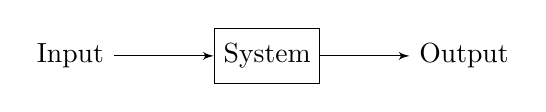
\begin{tikzpicture}[node distance=2.5cm,auto,>=latex']
	\node [input, align=center] (U) {Input};
	\node [block, align=center] (G) [right of=U] {System};
	\node [output, align=center] (y) [right of=G] {Output};
	\draw[->] (U) -- node {} (G);
	\draw[->] (G) -- node {} (y);
	\end{tikzpicture}
	
	or
	
	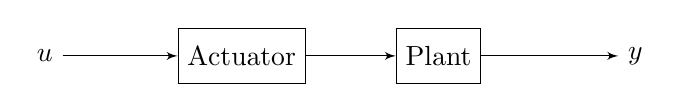
\begin{tikzpicture}[node distance=2.5cm,auto,>=latex']
		\node [input, align=center] (U) {$ u $};
		\node [block, align=center] (A) [right of=U] {Actuator};
		\node [block, align=center] (G) [right of=A] {Plant};
		\node [output, align=center] (y) [right of=G] {$ y $};
		\draw[->] (U) -- node {} (A);
		\draw[->] (A) -- node {} (G);
		\draw[->] (G) -- node {} (y);
	\end{tikzpicture}
\end{center}
For example, the ``plant'' could be something like a car, while the actuator would be the engine or motor driving the car.

A simplified block diagram of a feedback (closed-loop) system might look as follows, where:
\begin{itemize}
	\item $ r $ is the reference input
	\item $ e $ is the error signal
	\item $ u $ is the controlled input (control signal)
	\item $ y $ is the output
\end{itemize}
\begin{center}
	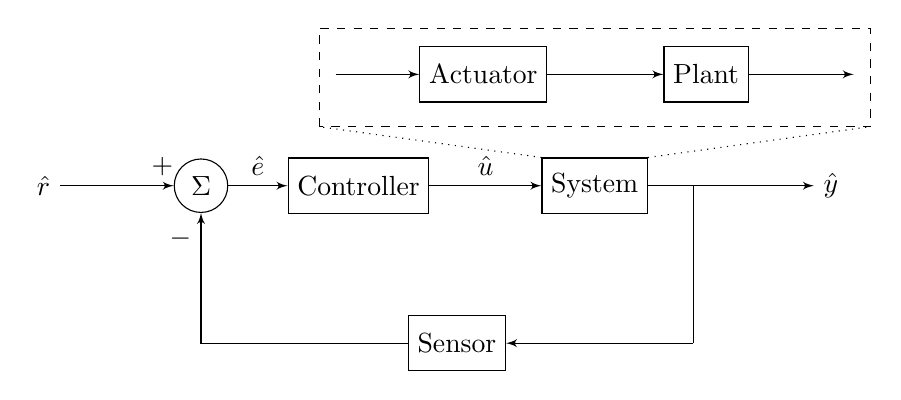
\begin{tikzpicture}[node distance=2.0cm,auto,>=latex']
	\node [input] (r) {$\hat{r}$};
	\node [sum] (sumr) [right of=r] {$\Sigma$};
	\node [block] (gc) [right of=sumr] {Controller};
	\node [block] (gp) [right of=gc,node distance=3.0cm] {System};
	\node [waypoint] (sumd) [right of=gp,node distance=1.25cm] {};
	\node [output] (y) [right of=sumd,node distance=1.75cm]{$\hat{y}$};
	\node [waypoint] (sumn) [below of=sumd] {};
	\node [block] (h) [left of=sumn,node distance=3cm] {Sensor};
	
	
	\node [block] (ga) [above left of=gp,node distance=2.0cm] {Actuator};
	\node [block] (gpp) [above right of=gp,node distance=2.0cm] {Plant};
	\node [output] (yt) [right of=gpp] {};
	\node [input] (ut) [left of=ga] {};
	\draw[->] (ut)--(ga);
	\draw[->] (ga)--(gpp);
	\draw[->] (gpp)--(yt);
	\draw[dashed] (3.5,0.75) rectangle (10.5,2);
	\draw[dotted] (gp.north east) -- (10.5,0.75);
	\draw[dotted] (gp.north west) -- (3.5,0.75);
	
	\draw[->] (r) -- node[pos=0.9] {$+$} (sumr);
	\draw[->] (sumr) -- node {$\hat{e}$} (gc);
	\draw[->] (gc) -- node {$\hat{u}$} (gp);
	\draw (gp) -- (sumd);
	\draw (sumd) -- (sumn);
	\draw[->] (sumd) -- (y);
	\draw[->] (sumn) -- (h);
	\draw[->] (h) -| node[pos=0.9] {$-$} (sumr);
	\end{tikzpicture}
\end{center}
\begin{itemize}
	\item A control system can have a single input and a single output (SISO)
	\item Or, it can have multiple inputs and outputs (MIMO)
\end{itemize}
Very often, it is possible to choose between open-looped and closed-loop design for a control system. In general,
\begin{itemize}
	\item Open-loop systems are simple and low-cost
	\item Closed-loop systems are more complex and cost more (they involve measurements/sensors and correction/compensators)
\end{itemize}

\section*{Why is feedback needed in some control systems?}
The principal reason is \textbf{uncertainty}.
\begin{itemize}
	\item Disturbances
	\item Uncertainty in the model of the controlled object
\end{itemize}

\subsection*{Example}
Speed control for a vehicle that has to go from Point A to Point B, following the path shown
\begin{center}
	\begin{tikzpicture}
	\node (A) at (0,0) {A};
	\node[waypoint] (C) at (4,0) {};
	\node (B) at (6,2) {B};
	\draw[-latex] (A)--(C)--(B);
	\end{tikzpicture}
\end{center}
Open loop design would be easy (and sufficient) of there were not disturbances, or all disturbances were known exactly. In reality, this is not possible. Feedback control would be needed if we want to be accurate.

\begin{center}
	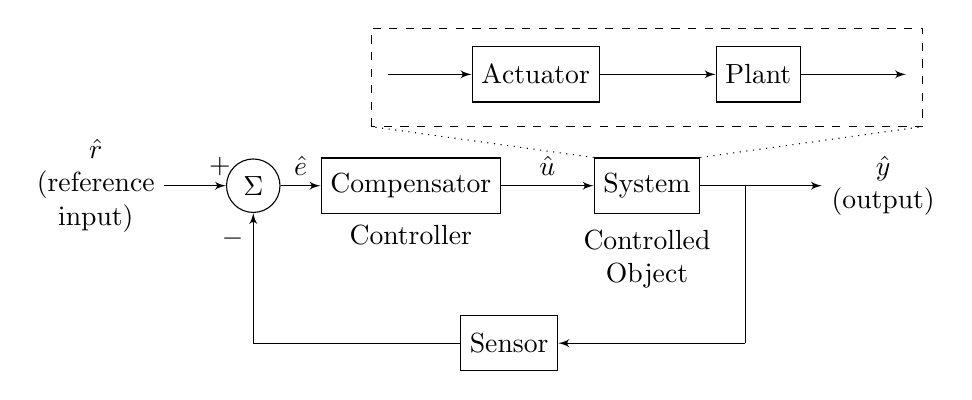
\begin{tikzpicture}[node distance=2.0cm,auto,>=latex']
	\node [input,align=center] (r) {$\hat{r}$\\(reference\\input)};
	\node [sum] (sumr) [right of=r] {$\Sigma$};
	\node [block] (gc) [right of=sumr] {Compensator};
	\node [block] (gp) [right of=gc,node distance=3.0cm] {System};
	\node [waypoint] (sumd) [right of=gp,node distance=1.25cm] {};
	\node [output,align=center] (y) [right of=sumd,node distance=1.75cm]{$\hat{y}$\\(output)};
	\node [waypoint] (sumn) [below of=sumd] {};
	\node [block] (h) [left of=sumn,node distance=3cm] {Sensor};
	
	\draw[->] (r) -- node[pos=0.9] {$+$} (sumr);
	\draw[->] (sumr) -- node {$\hat{e}$} (gc);
	\draw[->] (gc) -- node {$\hat{u}$} (gp);
	\draw (gp) -- (sumd);
	\draw (sumd) -- (sumn);
	\draw[->] (sumd) -- (y);
	\draw[->] (sumn) -- (h);
	\draw[->] (h) -| node[pos=0.9] {$-$} (sumr);
	
	\node [block] (ga) [above left of=gp,node distance=2.0cm] {Actuator};
	\node [block] (gpp) [above right of=gp,node distance=2.0cm] {Plant};
	\node [output] (yt) [right of=gpp] {};
	\node [input] (ut) [left of=ga] {};
	\draw[->] (ut)--(ga);
	\draw[->] (ga)--(gpp);
	\draw[->] (gpp)--(yt);
	\draw[dashed] (3.5,0.75) rectangle (10.5,2);
	\draw[dotted] (gp.north east) -- (10.5,0.75);
	\draw[dotted] (gp.north west) -- (3.5,0.75);
	
	\node[below of=gc,align=center,node distance = 0.625cm] {Controller};
	\node[below of=gp,align=center,node distance = 0.93125cm] {Controlled\\Object};
	\end{tikzpicture}
\end{center}
\begin{itemize}
	\item The compensator/controller takes the place of the human --- compensates for error.
	\item \textbf{The main objective of this course is the design of the compensator}.
\end{itemize}

\exmp
\paragraph*{Cruise Control for a Car:} Goals - maintain speed of a car at a prescribed value in the presence of external disturbances (\textbf{external forces such as wind gusts, gravitational forces on an incline, etc...}). Also - improve the dynamic response of the car as the driver ``steps on the gas''.
\paragraph*{(a)} Form a dynamic model of the car:
\begin{center}
	  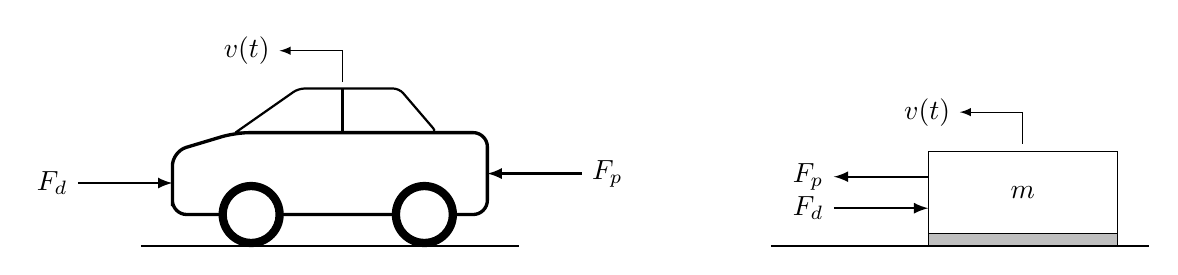
\begin{tikzpicture}[scale=0.8]
	\shade[top color=white, bottom color=white, shading angle={135}]
	[draw=black,fill=red!20,rounded corners=1.2ex,very thick] (1.5,.5) -- ++(0,1) -- ++(1,0.3) --  ++(3,0) -- ++(1,0) -- ++(0,-1.3) -- (1.5,.5) -- cycle;
	\draw[very thick, rounded corners=0.5ex,thick]  (2.5,1.8) -- ++(1,0.7) -- ++(1.6,0) -- ++(0.6,-0.7) -- (2.5,1.8);
	\draw[thick]  (4.2,1.8) -- (4.2,2.5);
	\draw[draw=black,fill=black,thick] (2.75,.5) circle (.5);
	\draw[draw=black,fill=black,thick] (5.5,.5) circle (.5);
	\draw[draw=black,fill=white,semithick] (2.75,.5) circle (.4);
	\draw[draw=black,fill=white,semithick] (5.5,.5) circle (.4);
	\draw[thick] (1,0) -- (7,0);
	\draw[thick,-latex] (0,1) node[left] {$ F_d $} -- ++(1.5,0);
	\draw[thick,-latex] (8,1.15) node[right] {$ F_p $} -- ++(-1.5,0);
	\draw[-latex] (4.2,2.6) |- ++(-1,0.5) node[left] {$ v(t) $};
	
	\begin{scope}[shift={(12cm,0cm)}]
	\draw[thick] (-1,0) -- (5,0);
	\draw[fill=gray!50] (1.5,0) rectangle (4.5,0.2);	
	\draw (1.5,0.2) rectangle node{$ m $} (4.5,1.5);
	\draw[thick,-latex] (0,0.6) node[left] {$ F_d $} -- ++(1.5,0);
	\draw[thick,latex-] (0,1.1) node[left] {$ F_p $} -- ++(1.5,0);
	\draw[-latex] (3,1.625) |- ++(-1,0.5) node[left] {$ v(t) $};
	
	\end{scope}
	\end{tikzpicture}
\end{center}
\begin{itemize}
	\item We are going to model the car as a simple lumped mass element $ m $, sliding on a viscous friction element $ F_B = Bv $ as a simplification of rolling resistance forces.
	\item Next, we assume two external forces acting on the car:
	\begin{itemize}
		\item $ F_p(t) $ - the propulsive force from the engine
		\item $ F_d(t) $ - the disturbance force from the environment
	\end{itemize}
	Also, assume $ F_p(t) = K_e \theta(t) $ where $ \theta(t) $ is the gas-pedal depression and $ K_e $ is a constant. Then from a simple force-balance:
	\[ m\frac{dv}{dt} + Bv = F_p(t) - F_d(t) \]
	\[ m\frac{dv}{dt} + Bv = K_e\theta(t) - F_d(t) \]
	This has the block diagram:
	\begin{center}	
		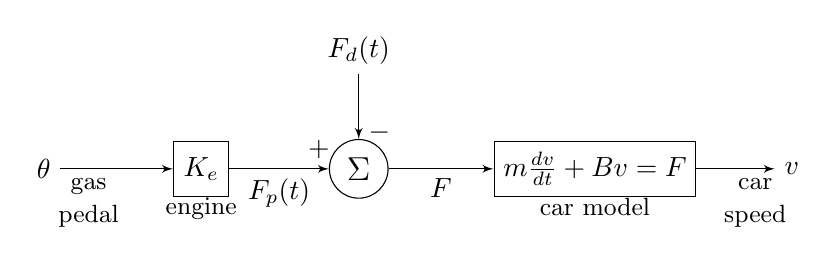
\begin{tikzpicture}[node distance=2cm,auto,>=latex']
		\node [input, align=center] (U) {$ \theta $};
		\node [block, align=center] (A) [right of=U] {$ K_e $};
		\node [sum, align=center] (S) [right of=A] {\large$ \Sigma $};
		\node [input, align=center] (D) [above of=S,node distance=1.5cm] {$ F_d(t) $};
		\node [block, align=center] (G) [right of=S,node distance=3cm] {$ m\frac{dv}{dt}+Bv=F $};
		\node [output, align=center] (y) [right of=G,node distance=2.5cm] {$ v $};
		\draw[->] (U) -- node[below,align=center,pos=0.25] {\small gas\\\small pedal} (A);
		\draw[->] (A) -- node[below] {$ F_p(t) $} node[above,pos=0.9] {$ + $} (S);
		\draw[->] (D) -- node[right,pos=0.9] {$ - $} (S);
		\draw[->] (S) -- node[below] {$ F $} (G);
		\draw[->] (G) -- node[below,align=center,pos=0.75] {\small car\\\small speed} (y);
		
		\node[below] at (2,-0.25) {\small engine};
		\node[below] at (7,-0.25) {\small car model};
		\end{tikzpicture}
	\end{center}
\end{itemize}
\paragraph*{(b)} Closed-loop Control: Now design a controller. Assume we will use error-based control. In other words, given a desired speed $ v_d $, and the measured car speed $ v(t) $, we define the error $ e(t) $ as 
\[ e(t) = v_d(t) - v(t) \]
and choose a control law that tells us to depress the gas pedal by an amount proportional to the error:
\[ \theta(t) = K_ce(t) = K_c(v_d(t)-v(t)), \]
so that the propulsive force acting on the car is
\[ F_p(t) = K_e\theta(t) = K_cK_e(v_d(t)-v(t)) \]
\begin{center}	
	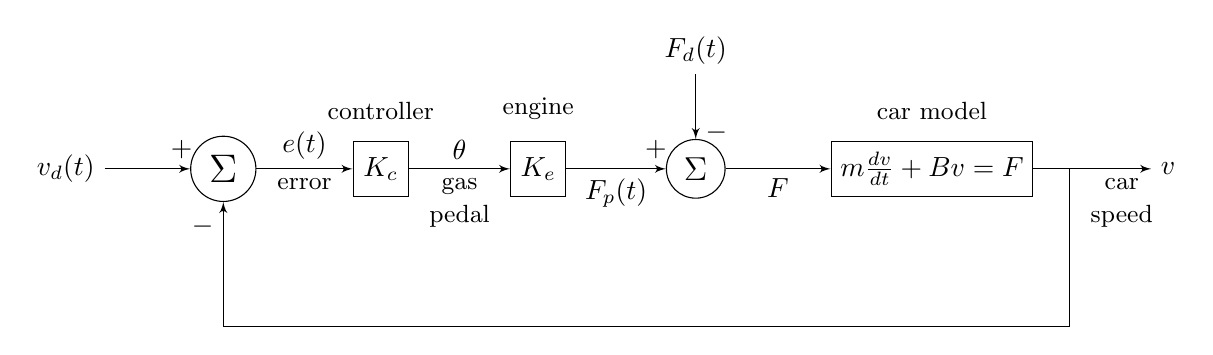
\begin{tikzpicture}[node distance=2cm,auto,>=latex']
	\node [input, align=center] (R) {$ v_d(t) $};
	\node [sum,right of=R] (SE) {\Large$ \Sigma $};
	\node [block,right of=SE] (C) {$ K_c $};
	\node [block, align=center] (A) [right of=C] {$ K_e $};
	\node [sum, align=center] (S) [right of=A] {\large$ \Sigma $};
	\node [input, align=center] (D) [above of=S,node distance=1.5cm] {$ F_d(t) $};
	\node [block, align=center] (G) [right of=S,node distance=3cm] {$ m\frac{dv}{dt}+Bv=F $};
	\node [output, align=center] (y) [right of=G,node distance=3cm] {$ v $};
	\node [waypoint] (wp) [right of=G,node distance=1.75cm] {};
	\node [waypoint] (H) [below of=S] {};
	
	\draw[->] (R) -- node[above,pos=0.9] {$ + $} (SE);
	\draw[->] (SE) -- node[below] {\small error} node[above] {$ e(t) $} (C);
	\draw[->] (C) -- node[below,align=center] {\small gas\\\small pedal} node[above] {$ \theta $} (A);
	\draw[->] (A) -- node[below] {$ F_p(t) $} node[above,pos=0.9] {$ + $} (S);
	\draw[->] (D) -- node[right,pos=0.9] {$ - $} (S);
	\draw[->] (S) -- node[below] {$ F $} (G);
	\draw[->] (G) -- node[below,align=center,pos=0.75] {\small car\\\small speed} (y);
	\draw[->] (wp) |- (H) -| node[left,pos=0.9] {$ - $} (SE);
	
	\node[above] at (4,0.5) {\small controller};
	\node[above] at (6,0.5) {\small engine};
	\node[above] at (11,0.5) {\small car model};
	\end{tikzpicture}
\end{center}
This is known as \textbf{\textit{proportional control}}.

\section*{Compensator Design}
The Big Picture:
\begin{itemize}
	\item We have an object (or system/plant) to control, and we are told what the system must be able to do.
	\item Principal steps in the controller design process:
	\begin{enumerate}
		\item We obtain a math model for the object or system to be controlled. In other words, a mathematical relationship between the input to the system and the output from the system. We need to understand the ``dynamics'' of the system.
		\item Use knowledge of control theory to come up with a mathematical representation of the controller or compensator (i.e. math relationship between the input to the controller and its output).
		\item Build a physical device that has the input-output relationship developed in (2) above. For example, a microcontroller to implement our control system.
	\end{enumerate}
	\item In this course, we concern ourselves with Step 2. Pencil and paper design, using mostly mathematics. 
\end{itemize}

Once again, the goal for this course is to learn how to design compenators. This is done in 3 phases:
\begin{enumerate}
	\item Learn how to characterize dynamic systems (review ENG 102, EME 171, etc...)
	\item Learn feedback principles (principles that govern feedback systems)
	\item Design methods
\end{enumerate}

\section*{Characterization of Dynamic Systems}
The input and output of a dynamic system are usually related by one or more differential equations. These equations can be obtained in a variety of ways.
\begin{itemize}
	\item Newton's laws ($ F=ma $) (mechanical systems)
	\item Lagrange Method
	\item Kirchoff's voltage/current laws (electrical systems)
	\item Bond graphs
	\item etc...
\end{itemize}
To do control work, we can (a) choose to work directly with such differential equations or (b) we can transform them first into algebraic equations using the Laplace Transform before proceeding with control work. In Case (a) we speak of the time-domain analysis (state-space approach), called ``modern control''. In Case (b) we speak of frequency-domain analysis (such as Bode or Nyquist plots), called ``classical control''. The main mathematical tool used in the second approach is the Laplace transform. We will thus start with a review of the Laplace transform.

\section*{Review of the Laplace Transform}
The Laplace transform converts a function of time $ f(t) $ into a function of a different variable $ s $, referred to as the Laplace variable. The reason this is useful is that it allows manipulation of ordinary differential equations (ODEs).
\begin{enumerate}
	\item The solution to ODEs is ``difficult'', so
	\item Transform the problem into a ``domain'' where the solution is easier.
	\item Solve the problem in the new domain.
	\item Perform the ``inverse'' transform to move the solution back to the original domain.
\end{enumerate}
\begin{center}
	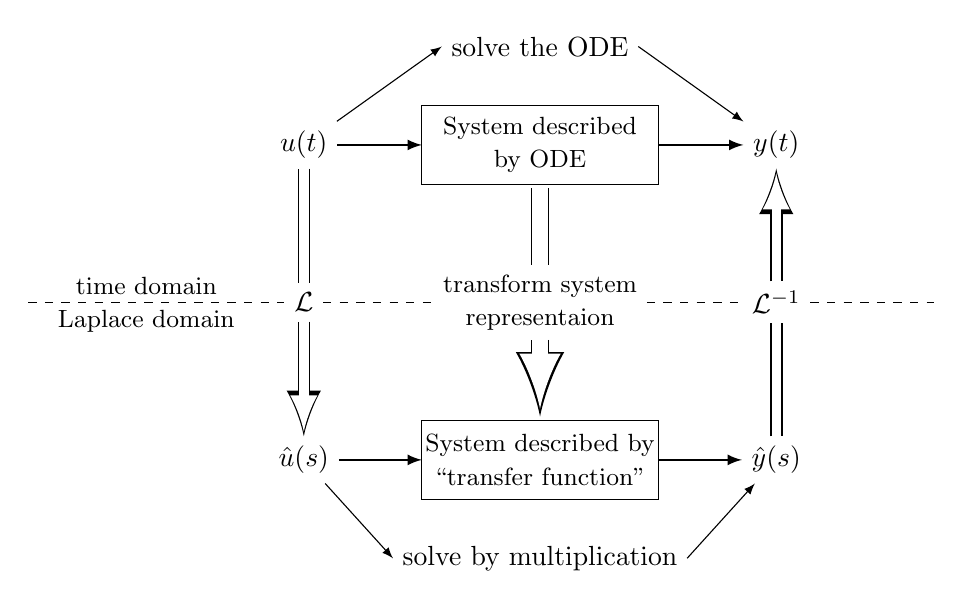
\begin{tikzpicture}
	\node (ut) at (0,2) {$ u(t) $};
	\node (yt) at (6,2) {$ y(t) $};
	\node (us) at (0,-2) {$ \hat{u}(s) $};
	\node (ys) at (6,-2) {$ \hat{y}(s) $};
	\node (LT) at (0,0) {$ \LT $};
	\node (LTn1) at (6,0) {$ \LT^{-1} $};
	\node (ODE) at (3,3.25) {solve the ODE};
	\node (Mult) at (3,-3.25) {solve by multiplication};
	\draw (1.5,1.5) rectangle node[align=center]{\small System described\\\small by ODE} (4.5,2.5);
	\draw (1.5,-1.5) rectangle node[align=center]{\small System described by\\\small ``transfer function''} (4.5,-2.5);
	\node[align=center] (C) at (3,0) {\small transform system\\\small representaion};
	
	\draw[-latex] (ut) -- (ODE.west);
	\draw[-latex] (ODE.east) -- (yt);
	\draw[-latex] (us) -- (Mult.west);
	\draw[-latex] (Mult.east) -- (ys);
	
	\draw[thick,-latex] (ut) -- (1.5,2);
	\draw[thick,-latex] (4.5,2) -- (yt);
	\draw[thick,-latex] (us) -- (1.5,-2);
	\draw[thick,-latex] (4.5,-2) -- (ys);
	
	
	\draw[line width=.16cm,-latex] (ut) -- (LT) -- (us);
	\draw[line width=.12cm,-latex,color=white] (ut) -- (LT) -- ([yshift=0.06cm]us.north);
	\draw[line width=.16cm,-latex] (ys) -- (LTn1) -- (yt);
	\draw[line width=.12cm,-latex,color=white] (ys) -- (LTn1) -- ([yshift=-0.06cm]yt.south);
	
	
	\draw[line width=.24cm,-latex] (3,1.45) -- (C) -- (3,-1.45);
	\draw[line width=.20cm,-latex,color=white] (3,1.45) -- (C) -- (3,-1.35);
	
	\node[align=center] (label) at (-2,-0.03125) {\small time domain\\ \small Laplace domain};
	
	\draw[dashed] (-3.5,0) -- (LT) -- (C) -- (LTn1) -- ++(2,0);
	
	\end{tikzpicture}
\end{center}
\begin{itemize}
	\item The main merit of the Laplace transform is that it converts differential equations to algebraic problems of polynomials and rational functions (ratios of polynomials).
	\item The main drawback is that the Laplace transform only works with linear, time-invariant (LTI) ODEs.
\end{itemize}
We are going to have to limit ourselves to the study of control systems that can be described by LTI ODEs. For example:
\[ a\ddot{x} + b\dot{x} + cx = 0 \]
\[ \alpha \dot{y} + \beta y = \delta \sin \omega t \]
where $ a $, $ b $, $ c $, $ \alpha $, $ \beta $, $ \delta $, $ \omega $ are all constants.

\subsection*{Definition}
Let $ f(t) $ be a function of time. The Laplace transform of $ f(t) $ is defined as
\[ \LT[f(t)] \triangleq \int_{0^-}^{\infty} e^{-st}f(t)dt = F(s) \]
where the integral exists (that is, has some finite value) and where $ 0^- $ is slightly before 0. The Laplace transform converts known functions of time to functions of $ s $. It turns out that it makes things easier to take the variable $ s $ to be complex: 
\[ s=\sigma+\jw \]
where $ j=\sqrt{-1} $. This is because the roots of a polynomial may be complex, and because we will later be interested in the frequency response of systems.

Let's clarify our terminology:
\begin{itemize}
	\item $ f(0^-) $: initial conditions
	\item $ f(0^+) $: initial value
\end{itemize}
Sometimes $ f(0^-) \neq f(0^+)  $. For example, the unit step function:
\[ 1(t) = \left\{\begin{array}{c c}
	1,&t\geq0\\0,&t<0
	\end{array}\right. \]
The step function if a mathematical idealization of a true physical signal, i.e. switches.

\exmp
The unit step.
\[ 1(t) = \left\{\begin{array}{c c}
1,&t\geq0\\0,&t<0
\end{array}\right. \]
\[ \LT [1(t)] = \int_{0^-}^{\infty} e^{-st}1(t)dt = \int_{0^-}^{\infty}e^{-st}dt = -\frac{1}{s}e^{-st}|_0^\infty = -\frac{1}{s}(0-1) = \frac{1}{s} \]

We would like to be able to plot $ F(s) $ just as we plot $ f(t) $. But, $ s $ is complex! So, we have to think of a way of drawing a picture of $ F(s) $ that is different from the usual way of plotting $ f(t) $. What is usually done is to plot where $ F(s) $ goes to infinity (poles) and where it goes to zero (zeros). This is called a pole-zero diagram. For example, a system with two poles and one zero might look like this:
\begin{center}
	\begin{tikzpicture}[scale=1]
	\draw (-5,0) -- (2,0) node[below left] {$ \sigma $};
	\draw (0,-1.5) -- (0,1.5) node[below left] {$ j\omega $};
	\node at (-4,0) {\Large$ \times $};
	\node at (-1,0) {\Large$ \times $};
	\node at (-2,0) {\Large$ \circ $};
	
	\node[align=left] at (-4,1.25) {\Large$ \circ $:\normalsize Zeros};
	\node[align=left] at (-4,0.875) {\Large$ \times $:\normalsize Poles};
	\end{tikzpicture}
\end{center}

When does $ F(s)=1/s $ for to zero? There is no \textbf{finite} zero. Obviously, when $ s\to\infty $, $F(s)\to0 $. So, there is a zero at infinity. But we don't worry about that in this course.

Next, let's clarify some issues concerning the Laplace Transform in general.
\begin{itemize}
	\item Recall the definition of $ F(s) = \int_{0^-}^{\infty} e^{-st}f(t)dt $
	\item $ F(s) $ has no information about $ f(t) $ before $ t=0 $. Only $ f(t) $ for $ t\geq 0$ is encoded in $ F(s) $. This is because of how $ F(s) $ is defined.
%	\item There is no one-to-one correspondence between $ \LT[f(t)] $ and $ f(t) $ --- no uniqueness --- unless we impose the restriction: $ f(t)=0 $ for $ t<0 $.
	\item Functions with such restrictions are often represented as ``causal'' functions. For example:
	\begin{center}
		\begin{tikzpicture}[scale=2]
		\draw[->] (-0.5,0) -- (2,0);  % x Axis
		\draw[->] (0,-0.25) -- (0,1.0);  % y Axis
		\node[below] at (1.9,0) {$ t $};
		\node[left] at (0,0.9) {$ f(t) $};
		\node[above] at (1,0.5) {$ e^{-t} $};
		
		\draw[domain=0:2] plot (\x,{.75*exp(-\x)});
		\end{tikzpicture}
	\end{center}
	We can write such a function in one of 2 ways:
	\[ f(t) = \left\{\begin{array}{c c}
	e^{-t},&t\geq0\\0,&t<0
	\end{array}\right. \]
	or more simply
	\[ f(t)=e^{-t}1(t) \]
	The initial condition is always zero for a causal function. So, we can talk of
	\begin{itemize}
		\item causal exponential (drawn above)
		\item causal ramp: $ f(t)=at\cdot1(t) $ where $ a $ is a constant
		\item causal sine: $ f(t)=a\sin(\wt)1(t) $ where $ a $ is a constant
		\item causal cosine: $ f(t)=a\cos(\wt)1(t) $ where $ a $ is a constant
		\item etc...
	\end{itemize}
	From now on, we will only take the LT of causal functions.
\end{itemize}

One other item if interest is the \textbf{Dirac Delta Function} $ \delta(t) $.  Consider the rectangle shown.
\begin{center}
	\begin{tikzpicture}
	\draw (-1.5,0) -- (3.5,0);  % x Axis
	\draw (0,-2.0) -- (0,2.0);  % y Axis
	\node[below] at (3.4,0) {$ t $};
	\node[left] at (0,1.8) {$ f(t) $};
	
	\draw (.5,0) |- (0,1);
	
	\node[below] at (0.5,0) {$ \tau $};
	\node[left] at (0,1) {$ 1/\tau $};
	
	\begin{scope}[shift={(6cm,0cm)}]
	\draw (-1.5,0) -- (3.5,0);  % x Axis
	\draw (0,-2.0) -- (0,2.0);  % y Axis
	\node[below] at (3.4,0) {$ t $};
	\node[left] at (0,1.8) {$ \delta(t) $};
	
	\draw[->,ultra thick] (0,0) -- (0,1.5);
	
	\node[right] at (0,1) {``Impulse''};
	\end{scope}
	\end{tikzpicture}
\end{center}
It's area is one. The delta function $ \delta(t) $ can be viewed as the area of this rectangle as $ \tau\to0 $. For a function $ f(t) $ as shown
\begin{center}
	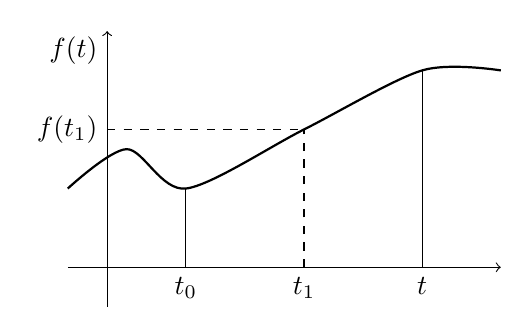
\begin{tikzpicture}
	
	%	\begin{scope}
	%	\clip [saveuse path={plot path}{plot [smooth] coordinates { (-0.5,1) (0.25,1.5) (1,1) (2.5,1.75) (4,2.5) (5,2.5)}}]
	%	|- (0,0) -- cycle;
	%	\clip[preaction={draw,fill=gray!50}] (1,0) rectangle (4,2.5);
	%	\end{scope}
	
	\draw[->] (-0.5,0) -- (5,0);  % x Axis
	\draw[->] (0,-0.5) -- (0,3);  % y Axis
	
	\draw (1,0) -- (1,1);
	\draw (4,0) -- (4,2.5);
	
	\node[below] at (1,0) {$ t_0 $};
	\node[below] at (4,0) {$ t $};
	\node[left] at (0,2.75) {$ f(t) $};
	
	\draw[thick] plot [smooth] coordinates { (-0.5,1) (0.25,1.5) (1,1) (2.5,1.75) (4,2.5) (5,2.5)};
	
	\draw[dashed] (2.5,0) -- (2.5,1.75);
	\node[below] at (2.5,0) {$ t_1 $};
	\draw[dashed] (0,1.75) -- (2.5,1.75);
	\node[left] at (0,1.75) {$ f(t_1) $};
	
	\end{tikzpicture}
\end{center}
It can be shown that
\[ \int_{t_0}^t f(t)\delta(t-t_1)dt = f(t_1) \]
This is called the shifting property of the delta function (from calculus). Then,
\[ \LT[\delta(t)]= \int_{0^-}^{\infty} e^{-st}\delta(t)dt = e^{-s\cdot0} = 1\]
Thus,
\[ \Rightarrow\quad \LT[\delta(t)]=1 \]

Some properties of the Laplace Transformation:
\[ \text{If } \LT[f(t)]=F(s) \text{ and } \LT[g(t)]=G(s) \text{ then} \]
\begin{enumerate}
	\item $ \LT[e^{-at}f(t)]=F(s+a) $ where $ a $ is constant (frequency shifting)
	\item $ \LT[tf(t)]=-\frac{d}{ds}F(s) $
	\item $ \LT[t^nf(t)]=(-1)^n\frac{d^n}{ds^n}F(s) $
	\item $ \LT[af(t)+bg(t)]=aF(s)+bG(s) $ where $ a $ and $ b $ are constant (linearity)
	\item $ \LT[\frac{d}{dt}f(t)]=sF(s)-f(0^-) $
	\item $ \LT[\frac{d^2}{dt^2}f(t)]=s^2F(s)-sf(0^-)-\frac{df}{dt}(0^-) $
	\item $ \LT[\frac{d^n}{dt^n}f(t)]=s^nF(s)-\sum_{k=1}^n s^{n-k}\frac{d^{k-1}f}{dt^{k-1}}(0^-) $
	\item $ \LT[\int_{0^-}^t f(\tau) d\tau]=\frac{F(s)}{s} $
	\item $ \LT[f(t-\tau)] = e^{-\tau s}F(s) $ (time shifting)
\end{enumerate}

\subsection*{Proof of the theorems}
Show that $ \LT[\frac{d}{dt}f(t)]=sF(s)-f(0^-) $:
\[ \LT[\frac{d}{dt}f(t)] = \int_{0^-}^{\infty} e^{-st}\frac{d}{dt}f(t)dt \]
We use integration by parts: $ u = e^{-st} $, $ du=-se^{-st} $, $ v=f(t) $, $ dv=\frac{df}{dt}(t) dt $. Recall that for integration by parts,
\[ d(uv) = du\cdot v + u\cdot dv \]
\[ udv = d(uv) - vdu \]
\[ \int_{c_1}^{c_2} udv = uv|_{c_1}^{c_2} - \int_{c_1}^{c_2} vdu \]
So,
\begin{align*}
\int_{0^-}^{\infty} e^{-st}\frac{d}{dt}f(t)dt&= e^{-st}f(t)\Big|_{0^-}^{\infty} -  \int_{0^-}^{\infty}-se^{-st}f(t)dt\\
&= 0 - f(0^-) + sF(s)\\
&= sF(s)-f(0^-)
\end{align*}

Armed with the result $ \LT[1(t)] = 1/s $ and together with these theorems, we are able to determine the Laplace transform of practically all the functions encountered in the study of LTI systems.

\exmp
\[ f(t) = 1-2t \]
Or more ``formally'':
\[ f(t) = 1(t) - 2t\cdot1(t) \]
Find $ F(s) $:
\[ F(s) = \frac{1}{s} - 2\left[ -\frac{d}{ds}\frac{1}{s} \right] = \frac{1}{s} - 2\frac{1}{s^2} \]
\[ F(s) = \frac{s-2}{s^2} \]

\exmp 
\[ \LT[e^{-at}1(t)] = \frac{1}{s+a} \]
\begin{center}
	\begin{tikzpicture}[scale=2]
	\draw[->] (-0.5,0) -- (2,0);  % x Axis
	\draw[->] (0,-0.25) -- (0,1.0);  % y Axis
	\node[below] at (1.9,0) {$ t $};
	\node[left] at (0,0.9) {$ f(t) $};
	\node[above] at (1,0.5) {$ e^{-at} $};
	
	\draw[domain=0:2] plot (\x,{.75*exp(-\x)});
	
	\begin{scope}[shift={(4.5cm,0.375cm)},scale=0.5]
	\draw (-3,0) -- (2,0) node[below left] {$ \sigma $};
	\draw (0,-1.5) -- (0,1.5) node[below left] {$ j\omega $};
	\node at (-1,0) {\Large$ \times $};
	\node[below] at (-1,0) {$ a $};
	%	\node at (-2,0) {\Large$ \circ $};
	\end{scope}
	
	\end{tikzpicture}
\end{center}

\exmp 
\[ \LT[t1(t)] = \frac{1}{s^2} \]
\begin{center}
	\begin{tikzpicture}[scale=2]
	\draw[->] (-0.5,0) -- (2,0);  % x Axis
	\draw[->] (0,-0.25) -- (0,1.0);  % y Axis
	\node[below] at (1.9,0) {$ t $};
	\node[left] at (0,0.9) {$ f(t) $};
	\node[above] at (1,0.5) {$ t $};
	
	\draw[domain=0:2] plot (\x,{.375*\x});
	
	\begin{scope}[shift={(4.5cm,0.375cm)},scale=0.5]
	\draw (-3,0) -- (2,0) node[below left] {$ \sigma $};
	\draw (0,-1.5) -- (0,1.5) node[below left] {$ j\omega $};
	\node at (0,0) {\Large$ \times $};
	\node[above right] at (0,0) {$ 2 $};
	%	\node at (-2,0) {\Large$ \circ $};
	\end{scope}
	
	\end{tikzpicture}
\end{center}

%\clearpage
%\noindent\begin{tikzpicture}[node distance=0.1cm]
%\node (a) {{\includegraphics[page=2,trim=2.54cm 4.75cm 1.75cm 8.5cm,clip]{MIT_OCW_CCexmp.pdf}}};
%\node[below=of a.south] (b) {{\includegraphics[page=3,trim=2.54cm 23.5cm 1.75cm 2.54cm,clip]{MIT_OCW_CCexmp.pdf}}};
%\end{tikzpicture}
%
%\noindent\begin{tikzpicture}[node distance=0.1cm]
%\node (a) {{\includegraphics[page=3,trim=2.54cm 6.25cm 1.75cm 6.25cm,clip]{MIT_OCW_CCexmp.pdf}}};
%\node[below=of a.south] (b) {{\includegraphics[page=4,trim=2.54cm 22.25cm 1.75cm 2.54cm,clip]{MIT_OCW_CCexmp.pdf}}};
%\end{tikzpicture}
%
%\noindent\begin{tikzpicture}
%\node (a) {{\includegraphics[page=4,trim=2.54cm 4.0625cm 1.75cm 8.0625cm,clip]{MIT_OCW_CCexmp.pdf}}};
%\node (b) at (0,-11.625cm) {{\includegraphics[page=5,trim=2.54cm 21.8125cm 1.75cm 2.625cm,clip]{MIT_OCW_CCexmp.pdf}}};
%\end{tikzpicture}
%
%\noindent\begin{tikzpicture}[node distance=0.1cm]
%\node (a) {{\includegraphics[page=5,trim=2.54cm 6.25cm 1.75cm 8.625cm,clip]{MIT_OCW_CCexmp.pdf}}};
%\node[below=of a.south] (b) {{\includegraphics[page=6,trim=2.54cm 22.25cm 1.75cm 2.54cm,clip]{MIT_OCW_CCexmp.pdf}}};
%\end{tikzpicture}
%
%\noindent\begin{tikzpicture}[node distance=0.1cm]
%\node (a) {{\includegraphics[page=6,trim=2.54cm 6.25cm 1.75cm 7.625cm,clip]{MIT_OCW_CCexmp.pdf}}};
%\node[below=of a.south] (b) {{\includegraphics[page=7,trim=2.54cm 22.25cm 1.75cm 2.54cm,clip]{MIT_OCW_CCexmp.pdf}}};
%\end{tikzpicture}

\end{document}